\documentclass[acmtog]{acmart}
% Title portion
\title{Fluid-Solid coupling using SPH method}
\author{Tianyuan Wu}

% Document starts
\begin{document}
\maketitle

\vspace*{2 ex}

\section{Introduction}
In this project, I use smooth particle hydrodynamics (SPH) method to simulate the two-way coupling of fluid and rigid bodies. 
SPH method is a particle based method which is widely used in fluid simulation. In this work, I implemented a fast, parallel 
SPH fluid simulator with real-time rendering and interaction. It contains 3 parts: (1) The fluid and rigid body simulator (solver); 
(2) User interaction handler; (3) Fluid and rigid body renderer (Third-Party library). The code were written in C++, 
with third party libraries \texttt{OpenGL}, \texttt{OpenMP}, \texttt{glm} and \texttt{splatter} used. A simple demo of 
my implementation is shown in Fig.1.
\begin{figure}[H]
    \centering
    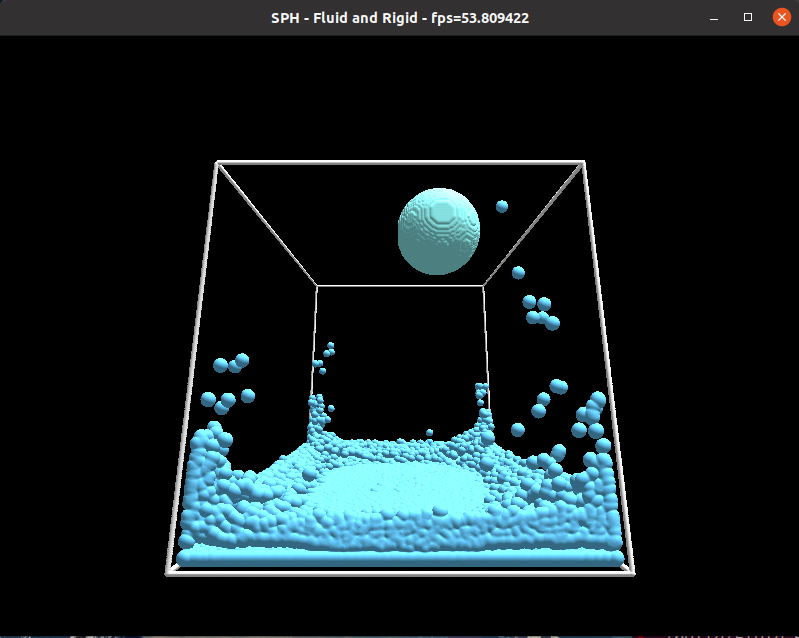
\includegraphics[scale=0.2]{../1.png}
    \caption{Demo of fluid simulation}
\end{figure}

\section{Implementation Details}
\subsection{SPH method}
In general, there are 2 approaches for fluid simulation, the Eulerian approach and Langrangian approach. The Eulerian 
approach usually divides the world into mesh grids, and use finite volume method or finite element method solver to 
calculate the force and velocity field in each mesh grid. But Langrangian methods consider fluid into discrete particles. 
Thus, the Naive-Stokes equation has different form in Eulerian and Langrangian approaches.\\
Smooth Particle Hydrodynamics (SPH) method is a particle based method (Langrangian approach). In this point of view, 
the dynamics of every particle in this system follows the equation:
$$\frac{D{\vec{u}}}{D{t}} + \frac{1}{\rho}\nabla p = \vec{g} + \nu \nabla \cdot \nabla \vec{u}$$
The other key idea of SPH is use the sum over all sample points to approximate the integral. 
$$f(x) = \int _{x'}(f(x')\omega _h(||x - x'||))dV \approx \sum_{i}f_i\omega_h(||x - x'||))V_i$$
Where $\omega_(r)$ is the kernel function. In 3D simulation, we usually use the Poly6 kernel:
$$\omega_{Poly6, h}(r) = \begin{cases}
    K_{Poly6}(h^2 - r^2)^3, \quad 0\le r \le h\\
    0, \quad otherwise \end{cases}
$$
Then, for some attribute $A$ of particle $i$, the influence of other particles to this particle is:
$$A(r) = \sum_{j}{A_j \frac{m_j}{\rho_j} W(\vec{r} - \vec{r}_j, h)}$$
We know, for a given particle, the acceleration can be calculated by the Newton's second law:
$$\vec{F} = \vec{F}^{ext} + \vec{F}^{pres} + \vec{F}^{visc} + \vec{F}^{surf} = \rho \vec{a}$$
Where $\vec{F}^{ext}$ is the external force (gravity), $\vec{F}^{pres}$ is the force caused by 
pressure, $\vec{F}^{visc}$ is the force caused by viscosity, and $\vec{F}^{surf}$ is the surface 
tension.\\
Finally, we can observe the discrete form of acceleration:
$$\vec{a}_i = \vec{a}_i^{pres} + \vec{a}_i^{visc} + \vec{a}_i^{surf} + \vec{g}$$
where
$$\vec{a}_i ^{pres} = m\frac{45}{\pi h^6}\sum_{j}(\frac{p_i + p_j}{2\rho _i \rho _j}(h-r)^2\frac{r_i - r_j}{|r_i - r_j|})$$
$$\vec{a}_i ^{visc} = m\mu\frac{45}{\pi h^6}\sum_{j}(\frac{\vec{u}_i - \vec{u}_j}{\rho_i \rho_j}(h - |r_i - r_j|))$$
$$\vec{a}_i ^{surf} = -\sigma\nabla ^2c_s \frac{\nabla c_s}{\rho_i |\nabla c_s|}$$
Hence, in the simulation, we just need to re-calculate the acceleration each step, and get the velocity and 
position by integration of $\vec{a}$. 

\subsection{Handle interaction between fluid and rigid}
In this work, a two-way coupling is implemented, which means, not only the fluid will influence the 
rigid body, rigid bodies will also influence fluid. \\
For particle-based simulation,the coupling is quite simple. When collision between rigid bodies and 
particles detected, update their velocity by the conservation of momentum. First, we calculate the 
relative velocity $v_{rel}$ of fluid particle and rigid bodies. Then, we can get the normal $\vec{n}$ 
of the the collision surface. $v_{rel}$ has 2 two compoents, one is parpendicular to the surface 
($v_{rel}\cos<v_{rel}, \vec{n}>$), the other is parallel to the surface ($v_{rel}\sin<v_{rel}, \vec{n}>$). 
The collision will only change the parpendicular compoent. Also, we can calculate the velocity change 
of the rigid body by conservation of momentum. This method works well in practice, we can observe the 
rigid body floating on the fluid if the density of rigid body is less the fluid.

\subsection{Reduction of complexity}
By what we've discussed, for evey particle, we need to re-calculate the force between it and all 
other particles which distance between it is less or equal than $r$ in each time step. But in 
naive implementation, finding all particles with $||r_i - r_j|| < r$ need to traverse all particles 
in the system. Hence, the time complexity of naive implementation of SPH method is $O(n^2)$ each time step 
($n$ is the number of particles in this system).\\
To reduce the complexity, there are many approaches, such as KD tree and spatial hash. In my implementation, 
a spatial hash table is build in each step. The basic idea is, we divide the world into many 
$(r\times r \times r)$ cube grids, and give each of them a key (index). 
$$HashKey(i, j, k) = i \cdot LEN_Y \cdot LEN_Z + j \cdot LEN_Z + k$$
The value of some key is a list of particles in this grid:
$$Table[HashKey(i, j, k)] = \{\text{Particles in grid (i, j, k)} \}$$
By this method, we can get the neighbor particles in $O(1)$ time on average. Hence, the average 
time complexity is reduced to $O(n)$ each step.

\subsection{Parallelism}
This work also contains other optimization of SPH method, including thread level parallelism and 
data level (ISA level) parallelism.\\
For thread level parallelism, we use \texttt{OpenMP} for acceleration. OpenMP (Open multi-processing) 
is a shared-memory multi-threading library. We can use simple \texttt{\#pragma} instructions to 
implemente parallelism. for example, \texttt{\#pragma omp parallel for} tolds the compiler to 
parallel the following for loop, and \texttt{\#pragma omp critical} tolds the compiler the following 
scope is a critical section. By this way, we can improve the multi-core performance.\\
For data (ISA) level parallelism, I use SIMD (single instruction multiple data-flows) technique in 
this project. The Intel AVX instrincs provides us a simple way to use AVX instructions, which can 
calculate 8 floating point operations in one cycle.\\
By these parallelism optimizations, the performance of my simulator improved significantly (It's
shown in Results part).

\subsection{Interaction and Rendering}
I implemented a real-time interaction between the simulator and user. We can use keyboard and mouse 
to control the system, here's a simple conclusion.\\
\texttt{
Key F: full view\\
Key N: normal of vertices\\
Key D: depth vies\\
Key Space: pause\\
Key Up: add particles to system\\
Key Down: Enable the ball drop down\\
Mouse cursor: change the direction of view\\
}
I use a third party library \texttt{splatter} for the rendering part, which is based on the paper ``Particle Splatting: 
Interactive Rendering of Particle-Based Simulation Data, Adams, B., Lenaerts, T. \& Dutre, P. (2006)''.
One demo of the rendering part is shown in Fig.2, and the github repo of it can be find at \texttt{https://github.com/MoleTrooper/splatter}
\begin{figure}[H]
    \centering
    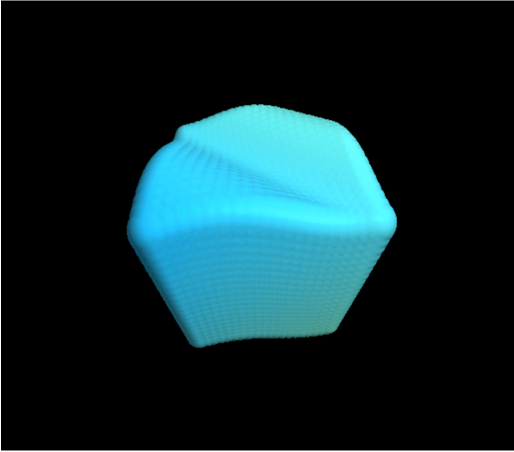
\includegraphics[scale=0.6]{../8.png}
    \caption{Render demo of Splatter}
\end{figure}

\section{Results}
\subsection{Simulation Result}
The implementation is tested on different system configurations, and the video of one demo is shown in the 
presentation slides, here's some snapshots of the demo system. In this demo, we use a blue ball (rigid) to 
test the coupling performance.
\begin{figure}[H]
    \centering
    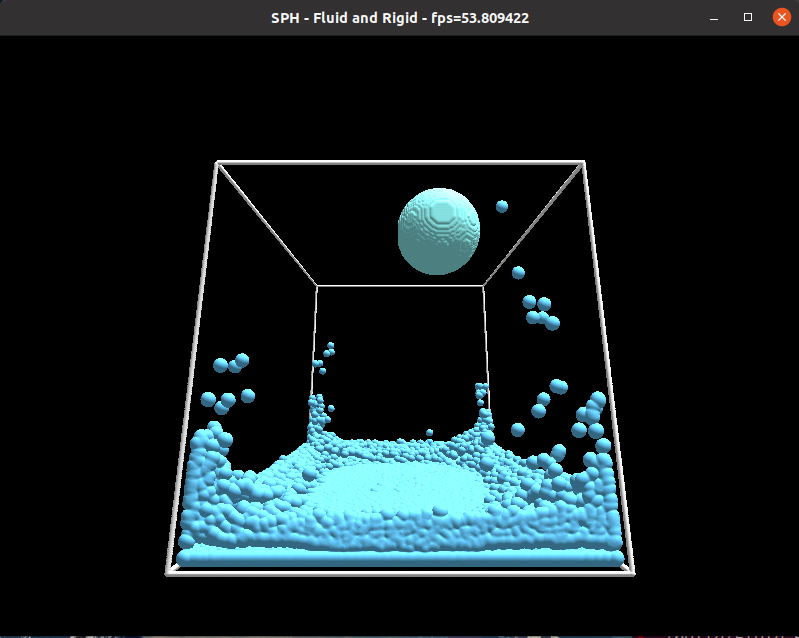
\includegraphics[scale=0.2]{../1.png}
    \caption{Add liquid into system (without ball)}
\end{figure}

\begin{figure}[H]
    \centering
    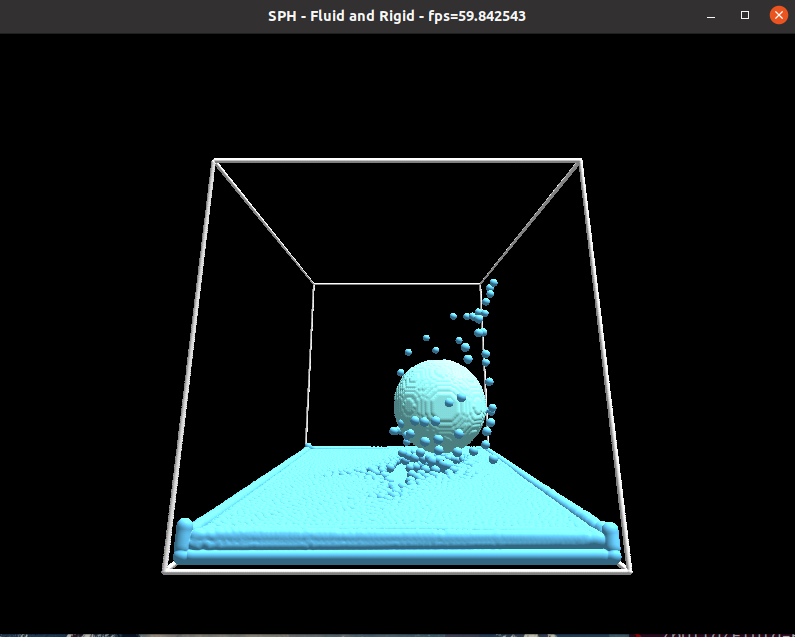
\includegraphics[scale=0.2]{../2.png}
    \caption{Interaction between ball and fluid - 1}
\end{figure}

\begin{figure}[H]
    \centering
    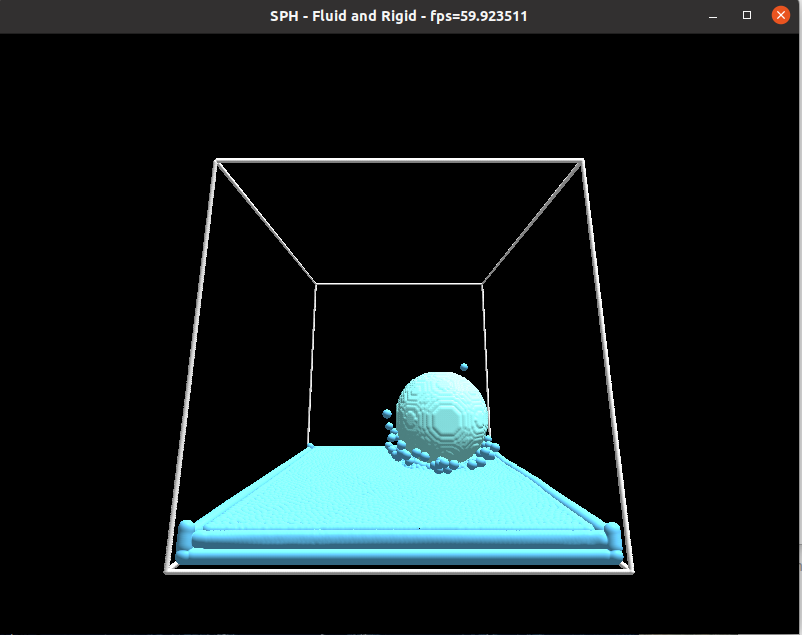
\includegraphics[scale=0.2]{../6.png}
    \caption{Interaction between ball and fluid - 2}
\end{figure}

\begin{figure}[H]
    \centering
    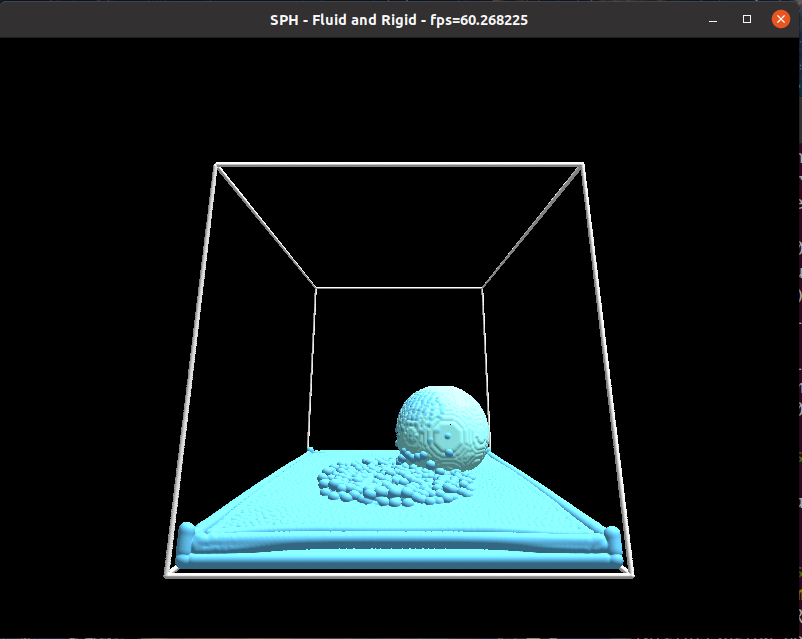
\includegraphics[scale=0.2]{../3.png}
    \caption{Add additional water into the system}
\end{figure}

\begin{figure}[H]
    \centering
    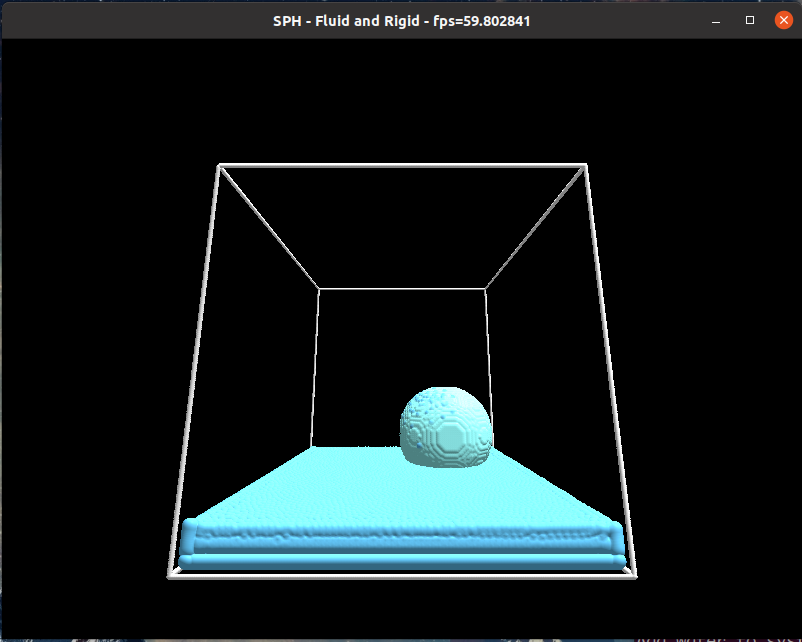
\includegraphics[scale=0.2]{../5.png}
    \caption{Ball-fluid system - stable}
\end{figure}

\subsection{Performance Evaluation}
I've also test the performance of this solver. The configuration of the evaluation platform is:\\
\texttt{
Ubuntu 20.04 LTS, GCC 9.2\\
OpenGL 3.3.0\\
Intel i7-8700k CPU(6 core, 12 threads)\\
16GB memory\\
}
We add about 20,000 particles and one rigid body into the system, and the performance is:
8-12 fps with 1 thread (no parallelism); 30-50 fps with 6 core, 12 threads.\\
Also, I use \texttt{htop} to monitoring CPU exploitation, the result is shown in Fig.8, 
which we can observe that almost all cores have 100\% exploitation.
\begin{figure}[H]
    \centering
    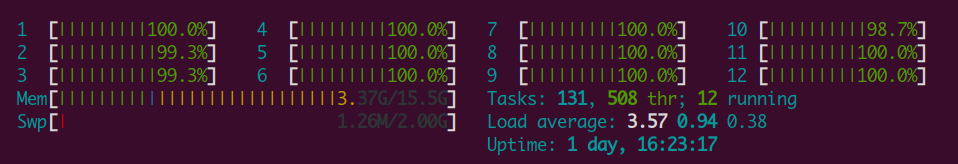
\includegraphics[scale=0.2]{../7.png}
    \caption{CPU exploitation}
\end{figure}

\end{document}
